% questions.tex —— 2017 年·天津卷·文科 · 题目内容片段（无答案）
% 由 tools/generate_projects.py 依来源总账自 2017/2017_数学真题_天津文_试题.md 生成，勿手改（改源 MD 后重跑）

\gkpart{数学}

\begin{gktip}
\textbf{来源说明}：本题面依据固定源 PDF 两页 A3 页面逐题核对，原卷印刷页码 1057–1058。固定源不附答案；本文件仅为题面规范源。
\end{gktip}

\gkpart{一、选择题}

\begin{question}
\gkti{1}
设集合 $A=\{1,2,6\}$，$B=\{2,4\}$，$C=\{1,2,3,4\}$，则 $(A\cup B)\cap C=$（　）

\begin{itemize}
\item (A) $\{2\}$
\item (B) $\{1,2,4\}$
\item (C) $\{1,2,4,6\}$
\item (D) $\{1,2,3,4,6\}$
\end{itemize}

\end{question}
\begin{question}
\gkti{2}
设 $x\in\mathbb R$，则“$2-x\geqslant0$”是“$|x-1|\leqslant1$”的（　）

\begin{itemize}
\item (A) 充分而不必要条件
\item (B) 必要而不充分条件
\item (C) 充要条件
\item (D) 既不充分也不必要条件
\end{itemize}

\end{question}
\begin{question}
\gkti{3}
有 5 支彩笔（除颜色外无差别），颜色分别为红、黄、蓝、绿、紫。从这 5 支彩笔中任取 2 支不同颜色的彩笔，则取出的 2 支彩笔中含有红色彩笔的概率为（　）

\begin{itemize}
\item (A) $\dfrac45$
\item (B) $\dfrac35$
\item (C) $\dfrac25$
\item (D) $\dfrac15$
\end{itemize}

\Needspace{0.4\textheight}
\end{question}
\begin{question}
\gkti{4}
阅读程序框图，运行相应的程序，若输入 $N$ 的值为 19，则输出 $N$ 的值为（　）
\nopagebreak[4]
\begin{center}\begin{tikzpicture}[>=stealth,thick,
  term/.style={draw,rounded corners=3pt,minimum width=21mm,minimum height=7mm},
  proc/.style={draw,minimum width=28mm,minimum height=8mm,align=center},
  test/.style={draw,diamond,aspect=2.35,inner sep=1pt,align=center},
  io/.style={draw,trapezium,trapezium left angle=70,trapezium right angle=110,
    minimum width=25mm,minimum height=8mm,align=center}]
  \node[term] (start) at (0,0) {开始};
  \node[io] (input) at (0,-1.15) {输入 $N$};
  \node[test] (div) at (0,-2.65) {$N$ 能被 $3$ 整除？};
  \node[proc] (divide) at (-2.9,-4.5) {$N=N/3$};
  \node[proc] (minus) at (2.9,-4.5) {$N=N-1$};
  \node[test] (small) at (0,-5.55) {$N\leq 3$？};
  \node[io] (output) at (0,-7.05) {输出 $N$};
  \node[term] (stop) at (0,-8.2) {结束};
  \draw[->] (start)--(input);
  \draw[->] (input)--(div);
  \draw[->] (div.south)--(0,-3.8)--(-2.9,-3.8)--(divide.north);
  \node at (.38,-3.55) {是};
  \draw[->] (div.east)--node[above]{否} ++(1.0,0)|-(minus.north);
  \draw[->] (divide.south)|-(small.west);
  \draw[->] (minus.south)|-(small.east);
  \draw[->] (small.south)--node[right]{是}(output.north);
  \draw[->] (output)--(stop);
  \draw[->] (small.west)--(-3.8,-5.55)--node[pos=.78,left]{否}(-3.8,-2.65)--(div.west);
\end{tikzpicture}
\end{center}
\nopagebreak[4]
\begin{itemize}
\item (A) 0
\item (B) 1
\item (C) 2
\item (D) 3
\end{itemize}

\end{question}
\begin{question}
\gkti{5}
已知双曲线 $\dfrac{x^2}{a^2}-\dfrac{y^2}{b^2}=1$（$a>0,b>0$）的右焦点为 $F$，点 $A$ 在双曲线的渐近线上，$\triangle OAF$ 是边长为 2 的等边三角形（$O$ 为原点），则双曲线方程为（　）

\begin{itemize}
\item (A) $\dfrac{x^2}{4}-\dfrac{y^2}{12}=1$
\item (B) $\dfrac{x^2}{12}-\dfrac{y^2}{4}=1$
\item (C) $\dfrac{x^2}{3}-y^2=1$
\item (D) $x^2-\dfrac{y^2}{3}=1$
\end{itemize}

\end{question}
\begin{question}
\gkti{6}
已知奇函数 $f(x)$ 在 $\mathbb R$ 上是增函数。若 $a=-f\left(\log_2\dfrac15\right)$，$b=f(\log_2 4.1)$，$c=f(2^{0.8})$，则 $a,b,c$ 的大小关系为（　）

\begin{itemize}
\item (A) $a<b<c$
\item (B) $b<a<c$
\item (C) $c<b<a$
\item (D) $c<a<b$
\end{itemize}

\end{question}
\begin{question}
\gkti{7}
设函数 $f(x)=2\sin(\omega x+\varphi)$，$x\in\mathbb R$，其中 $\omega>0$，$|\varphi|<\pi$。若 $f\left(\dfrac{5\pi}{8}\right)=2$，$f\left(\dfrac{11\pi}{8}\right)=0$，且 $f(x)$ 的最小正周期大于 $2\pi$，则（　）

\begin{itemize}
\item (A) $\omega=\dfrac23,\ \varphi=\dfrac{\pi}{12}$
\item (B) $\omega=\dfrac23,\ \varphi=-\dfrac{11\pi}{12}$
\item (C) $\omega=\dfrac13,\ \varphi=-\dfrac{11\pi}{24}$
\item (D) $\omega=\dfrac13,\ \varphi=\dfrac{7\pi}{24}$
\end{itemize}

\end{question}
\begin{question}
\gkti{8}
\Needspace{5\baselineskip}
已知函数

\nopagebreak[4]
\[
f(x)=\begin{cases}|x|+2,&x<1,\\x+\dfrac2x,&x\geqslant1.\end{cases}
\]

设 $a\in\mathbb R$，若关于 $x$ 的不等式 $f(x)\geqslant\left|\dfrac x2+a\right|$ 在 $\mathbb R$ 上恒成立，则 $a$ 的取值范围是（　）

\begin{itemize}
\item (A) $[-2,2]$
\item (B) $[-2\sqrt3,2]$
\item (C) $[-2,2\sqrt3]$
\item (D) $[-2\sqrt3,2\sqrt3]$
\end{itemize}

\end{question}
\gkpart{二、填空题}

\begin{question}
\gkti{9}
已知 $a\in\mathbb R$，$\mathrm i$ 为虚数单位，若 $\dfrac{a-\mathrm i}{2+\mathrm i}$ 为实数，则 $a$ 的值为 \gkblank{}。

\end{question}
\begin{question}
\gkti{10}
已知 $a\in\mathbb R$，设函数 $f(x)=ax-\ln x$ 的图象在点 $(1,f(1))$ 处的切线为 $l$，则 $l$ 在 $y$ 轴上的截距为 \gkblank{}。

\end{question}
\begin{question}
\gkti{11}
已知一个正方体的所有顶点在一个球面上，若这个正方体的表面积为 18，则这个球的体积为 \gkblank{}。

\end{question}
\begin{question}
\gkti{12}
设抛物线 $y^2=4x$ 的焦点为 $F$，准线为 $l$。已知点 $C$ 在 $l$ 上，以 $C$ 为圆心的圆与 $y$ 轴的正半轴相切于点 $A$。若 $\angle FAC=120^\circ$，则圆的方程为 \gkblank{}。

\end{question}
\begin{question}
\gkti{13}
若 $a,b\in\mathbb R$，$ab>0$，则 $\dfrac{a^4+4b^4+1}{ab}$ 的最小值为 \gkblank{}。

\end{question}
\begin{question}
\gkti{14}
在 $\triangle ABC$ 中，$\angle A=60^\circ$，$AB=3$，$AC=2$。若 $\overrightarrow{BD}=2\overrightarrow{DC}$，$\overrightarrow{AE}=\lambda\overrightarrow{AC}-\overrightarrow{AB}$（$\lambda\in\mathbb R$），且 $\overrightarrow{AD}\cdot\overrightarrow{AE}=-4$，则 $\lambda$ 的值为 \gkblank{}。

\end{question}
\gkpart{三、解答题}

\begin{question}
\gkti{15}
在 $\triangle ABC$ 中，内角 $A,B,C$ 所对的边分别为 $a,b,c$。已知 $a\sin A=4b\sin B$，$ac=\sqrt5\,(a^2-b^2-c^2)$。

(1)   求 $\cos A$ 的值；

(2)   求 $\sin(2B-A)$ 的值。

\end{question}
\begin{question}
\gkti{16}
电视台播放甲、乙两套连续剧，每次播放连续剧时，需要播放广告。已知每次播放甲、乙两套连续剧时，连续剧播放时长、广告播放时长、收视人次如下表所示：

【表 T16，原表数据转录】

\begin{center}
\begin{tabular}{lrrr}
\toprule
 & 连续剧播放时长（分钟） & 广告播放时长（分钟） & 收视人次（万） \\
\midrule
甲 & 70 & 5 & 60 \\
乙 & 60 & 5 & 25 \\
\bottomrule
\end{tabular}
\end{center}

已知电视台每周安排的甲、乙连续剧的总播放时间不多于 600 分钟，广告的总播放时间不少于 30 分钟，且甲连续剧播放的次数不多于乙连续剧播放次数的 2 倍。分别用 $x,y$ 表示每周计划播出的甲、乙两套连续剧的次数。

(1)   用 $x,y$ 列出满足题目条件的数学关系式，并画出相应的平面区域；

(2)   问电视台每周播出甲、乙两套连续剧各多少次，才能使总收视人次最多？

\Needspace{0.4\textheight}
\end{question}
\begin{question}
\gkti{17}
如图，在四棱锥 $P-ABCD$ 中，$AD\perp\text{\text{平面} }PDC$，$AD\parallel BC$，$PD\perp PB$，$AD=1$，$BC=3$，$CD=4$，$PD=2$。

(1)   求异面直线 $AP$ 与 $BC$ 所成角的余弦值；

(2)   求证：$PD\perp\text{\text{平面} }PBC$；

(3)   求直线 $AB$ 与平面 $PBC$ 所成角的正弦值。
\nopagebreak[4]
\begin{center}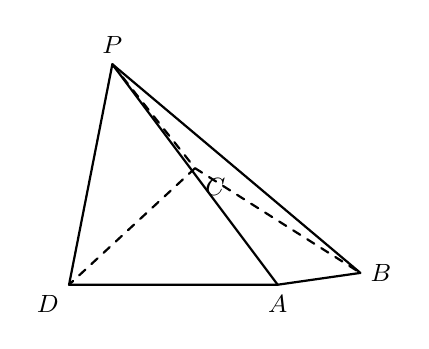
\begin{tikzpicture}[thick,line cap=round,line join=round,
  every node/.style={font=\small}]
  \coordinate (P) at (0,2.8);
  \coordinate (D) at (-.55,0);
  \coordinate (A) at (2.1,0);
  \coordinate (B) at (3.15,.15);
  \coordinate (C) at (1.05,1.48);
  \draw (P)--(D)--(A)--(B)--(P);
  \draw (P)--(A);
  \draw[dashed] (P)--(C) (C)--(D) (C)--(B);
  \node[above] at (P) {$P$};
  \node[below left] at (D) {$D$};
  \node[below] at (A) {$A$};
  \node[right] at (B) {$B$};
  \node[below right] at (C) {$C$};
\end{tikzpicture}
\end{center}
\nopagebreak[4]
\end{question}
\begin{question}
\gkti{18}
已知 $\{a_n\}$ 为等差数列，前 $n$ 项和为 $S_n$（$n\in\mathbb N^*$），$\{b_n\}$ 是首项为 2 的等比数列，且公比大于 0，$b_2+b_3=12$，$b_3=a_4-2a_1$，$S_{11}=11b_4$。

(1)   求 $\{a_n\}$ 和 $\{b_n\}$ 的通项公式；

(2)   求数列 $\{a_{2n}b_n\}$ 的前 $n$ 项和（$n\in\mathbb N^*$）。

\end{question}
\begin{question}
\gkti{19}
设 $a,b\in\mathbb R$，$|a|\leqslant1$。已知函数 $f(x)=x^3-6x^2-3a(a-4)x+b$，$g(x)=\mathrm e^x f(x)$。

(1)   求 $f(x)$ 的单调区间；

(2)   已知函数 $y=g(x)$ 和 $y=\mathrm e^x$ 的图象在公共点 $(x_0,y_0)$ 处有相同的切线。

① 求证：$f(x)$ 在 $x=x_0$ 处的导数等于 0；

② 若关于 $x$ 的不等式 $g(x)\leqslant\mathrm e^x$ 在区间 $[x_0-1,x_0+1]$ 上恒成立，求 $b$ 的取值范围。

\end{question}
\begin{question}
\gkti{20}
已知椭圆 $\dfrac{x^2}{a^2}+\dfrac{y^2}{b^2}=1$（$a>b>0$）的左焦点为 $F(-c,0)$，右顶点为 $A$，点 $E$ 的坐标为 $(0,c)$，$\triangle EFA$ 的面积为 $\dfrac{b^2}{2}$。

(1)   求椭圆的离心率；

(2)   设点 $Q$ 在线段 $AE$ 上，$|FQ|=\dfrac32c$，延长线段 $FQ$ 与椭圆交于点 $P$，点 $M,N$ 在 $x$ 轴上，$PM\parallel QN$，且直线 $PM$ 与直线 $QN$ 间的距离为 $c$，四边形 $PQNM$ 的面积为 $3c$。

① 求直线 $FP$ 的斜率；

② 求椭圆的方程。

\end{question}